% Original author-drawn map. Representative selection; no causal or citation edges.
% Institution name badges are verified affiliations, not official logos.
\documentclass[tikz,border=5pt]{standalone}
\usepackage[T1]{fontenc}
\usepackage{lmodern}
\usepackage{tikz}
\usetikzlibrary{calc,arrows.meta}
\definecolor{navy}{HTML}{162F4C}
\definecolor{ink}{HTML}{253A53}
\definecolor{muted}{HTML}{67778B}
\definecolor{rule}{HTML}{DCE5EE}
\definecolor{layout}{HTML}{2B7CAC}
\definecolor{poster}{HTML}{CA6A58}
\definecolor{artifact}{HTML}{2D8B73}
\definecolor{document}{HTML}{8064AD}
\definecolor{gan}{HTML}{C06849}
\definecolor{latent}{HTML}{647F9E}
\definecolor{diff}{HTML}{2675B4}
\definecolor{agent}{HTML}{775BAE}
\definecolor{struct}{HTML}{268B7B}
\definecolor{edit}{HTML}{AF4877}
\newcommand{\MapPaper}[8]{%
  \node[anchor=north west,draw=#7,fill=white,rounded corners=2pt,line width=.80pt,
   text width=3.12cm,inner xsep=4.1pt,inner ysep=3pt,align=left]
   at (#5,#6) {{\bfseries\fontsize{7.3}{8.1}\selectfont #2}\hfill
   {\fontsize{6.2}{7}\selectfont '#3}\\[-1pt]
   {\color{muted}\fontsize{6.35}{7.1}\selectfont #8}};%
}
\begin{document}
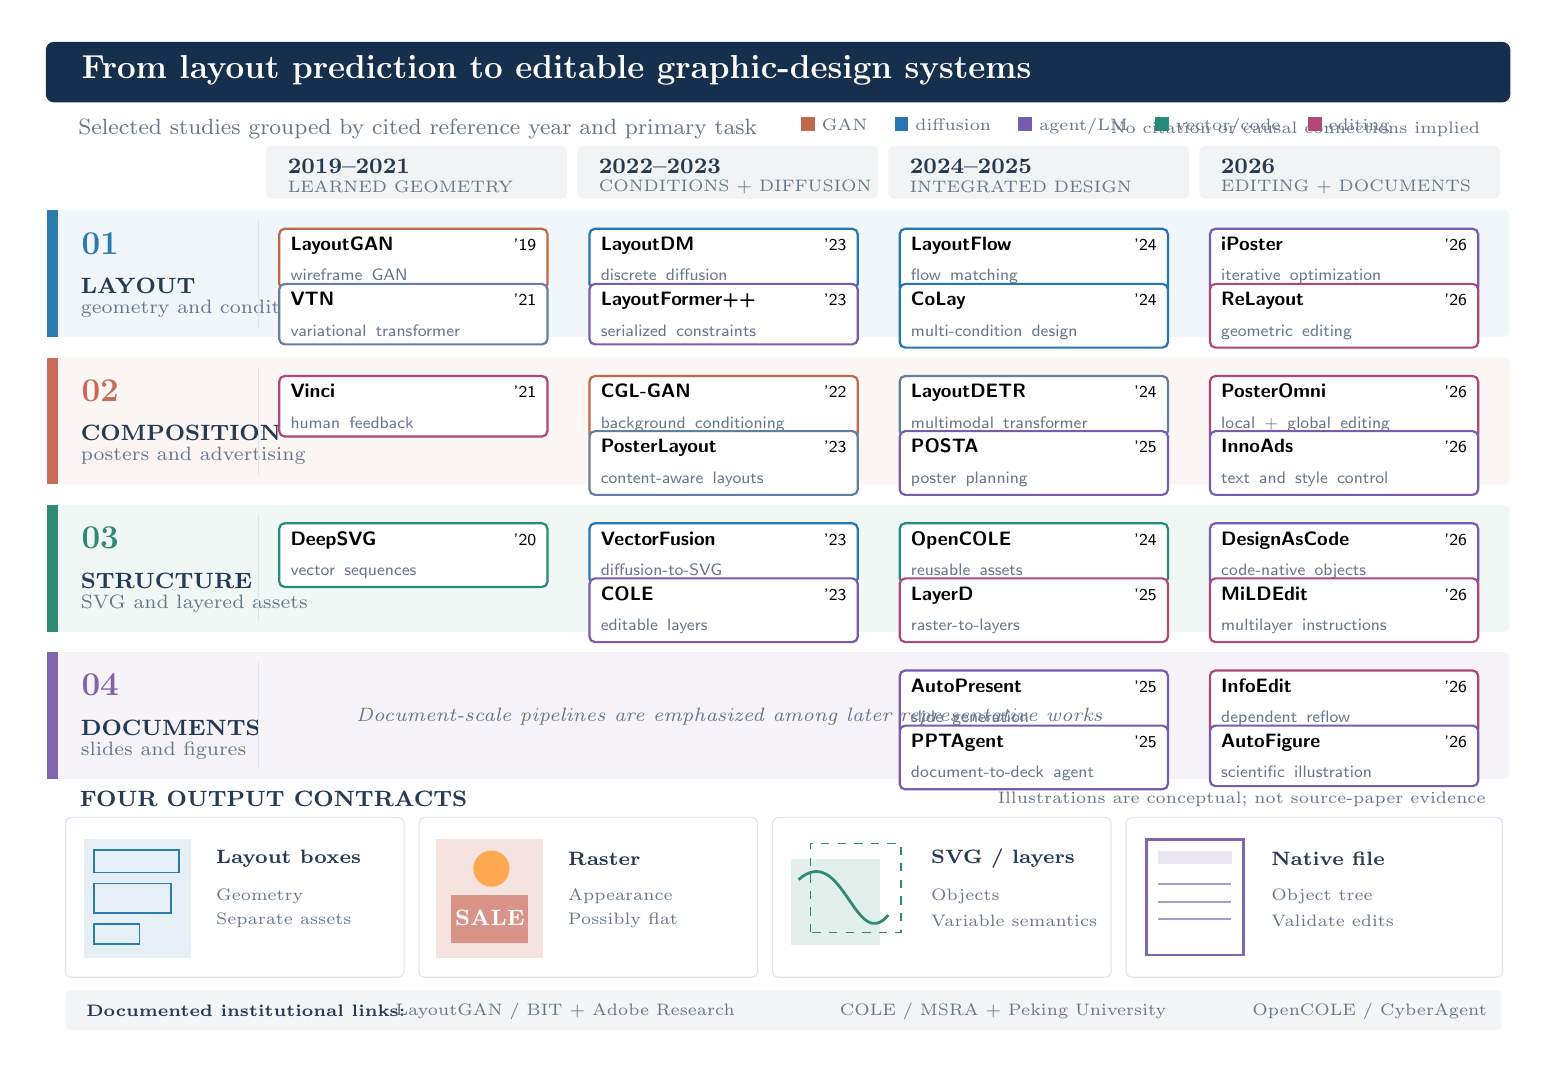
\begin{tikzpicture}[x=1cm,y=1cm,font=\sffamily]
\fill[white] (0,0) rectangle (19.08,13.0);
\fill[navy,rounded corners=3pt] (.23,12.05) rectangle (18.83,12.82);
\node[anchor=west,text=white,font=\bfseries\fontsize{13}{14}\selectfont] at (.56,12.46) {From layout prediction to editable graphic-design systems};
\node[anchor=west,text=muted,font=\fontsize{8}{9}\selectfont] at (.52,11.71) {Selected studies grouped by cited reference year and primary task};
\node[anchor=east,text=muted,font=\fontsize{6.0}{7}\selectfont] at (18.57,11.71) {No citation or causal connections implied};
\fill[navy!6,rounded corners=2pt] (3.03,10.83) rectangle (6.85,11.50);
\node[anchor=west,text=ink,font=\bfseries\fontsize{8.4}{9.2}\selectfont] at (3.18,11.24) {2019--2021};
\node[anchor=west,text=muted,font=\fontsize{6.0}{7}\selectfont] at (3.18,10.98) {LEARNED GEOMETRY};
\fill[navy!6,rounded corners=2pt] (6.98,10.83) rectangle (10.8,11.50);
\node[anchor=west,text=ink,font=\bfseries\fontsize{8.4}{9.2}\selectfont] at (7.13,11.24) {2022--2023};
\node[anchor=west,text=muted,font=\fontsize{6.0}{7}\selectfont] at (7.13,10.98) {CONDITIONS + DIFFUSION};
\fill[navy!6,rounded corners=2pt] (10.93,10.83) rectangle (14.75,11.50);
\node[anchor=west,text=ink,font=\bfseries\fontsize{8.4}{9.2}\selectfont] at (11.08,11.24) {2024--2025};
\node[anchor=west,text=muted,font=\fontsize{6.0}{7}\selectfont] at (11.08,10.98) {INTEGRATED DESIGN};
\fill[navy!6,rounded corners=2pt] (14.88,10.83) rectangle (18.7,11.50);
\node[anchor=west,text=ink,font=\bfseries\fontsize{8.4}{9.2}\selectfont] at (15.03,11.24) {2026};
\node[anchor=west,text=muted,font=\fontsize{6.0}{7}\selectfont] at (15.03,10.98) {EDITING + DOCUMENTS};
\fill[layout!7,rounded corners=2pt] (.25,9.07) rectangle (18.82,10.68);
\fill[layout] (.25,9.07) rectangle (.38,10.68);
\node[anchor=north west,text=layout,font=\bfseries\fontsize{12}{13}\selectfont] at (.56,10.52) {01};
\node[anchor=west,text=ink,font=\bfseries\fontsize{8}{9}\selectfont] at (.55,9.72) {LAYOUT};
\node[anchor=west,text=muted,font=\fontsize{6.8}{7.5}\selectfont] at (.55,9.43) {geometry and conditions};
\draw[rule] (2.93,9.19)--(2.93,10.56);
\fill[poster!7,rounded corners=2pt] (.25,7.2) rectangle (18.82,8.81);
\fill[poster] (.25,7.2) rectangle (.38,8.81);
\node[anchor=north west,text=poster,font=\bfseries\fontsize{12}{13}\selectfont] at (.56,8.65) {02};
\node[anchor=west,text=ink,font=\bfseries\fontsize{8}{9}\selectfont] at (.55,7.85) {COMPOSITION};
\node[anchor=west,text=muted,font=\fontsize{6.8}{7.5}\selectfont] at (.55,7.56) {posters and advertising};
\draw[rule] (2.93,7.32)--(2.93,8.69);
\fill[artifact!7,rounded corners=2pt] (.25,5.33) rectangle (18.82,6.94);
\fill[artifact] (.25,5.33) rectangle (.38,6.94);
\node[anchor=north west,text=artifact,font=\bfseries\fontsize{12}{13}\selectfont] at (.56,6.78) {03};
\node[anchor=west,text=ink,font=\bfseries\fontsize{8}{9}\selectfont] at (.55,5.98) {STRUCTURE};
\node[anchor=west,text=muted,font=\fontsize{6.8}{7.5}\selectfont] at (.55,5.69) {SVG and layered assets};
\draw[rule] (2.93,5.45)--(2.93,6.82);
\fill[document!7,rounded corners=2pt] (.25,3.46) rectangle (18.82,5.07);
\fill[document] (.25,3.46) rectangle (.38,5.07);
\node[anchor=north west,text=document,font=\bfseries\fontsize{12}{13}\selectfont] at (.56,4.91) {04};
\node[anchor=west,text=ink,font=\bfseries\fontsize{8}{9}\selectfont] at (.55,4.11) {DOCUMENTS};
\node[anchor=west,text=muted,font=\fontsize{6.8}{7.5}\selectfont] at (.55,3.82) {slides and figures};
\draw[rule] (2.93,3.58)--(2.93,4.95);
\MapPaper{A}{LayoutGAN}{19}{layoutgan2019}{3.18}{10.46}{gan}{wireframe GAN}
\MapPaper{A}{VTN}{21}{vtn2021}{3.18}{9.76}{latent}{variational transformer}
\MapPaper{A}{LayoutDM}{23}{layoutdm2023}{7.12}{10.46}{diff}{discrete diffusion}
\MapPaper{A}{LayoutFormer++}{23}{layoutformerpp2023}{7.12}{9.76}{agent}{serialized constraints}
\MapPaper{A}{LayoutFlow}{24}{layoutflow2024}{11.06}{10.46}{diff}{flow matching}
\MapPaper{A}{CoLay}{24}{colay2024}{11.06}{9.76}{diff}{multi-condition design}
\MapPaper{A}{iPoster}{26}{iposter2026}{15.00}{10.46}{agent}{iterative optimization}
\MapPaper{A}{ReLayout}{26}{relayoutedit2026}{15.00}{9.76}{edit}{geometric editing}
\MapPaper{B}{Vinci}{21}{vinci2021}{3.18}{8.59}{edit}{human feedback}
\MapPaper{B}{CGL-GAN}{22}{cglgan2022}{7.12}{8.59}{gan}{background conditioning}
\MapPaper{B}{PosterLayout}{23}{posterlayout2023}{7.12}{7.89}{latent}{content-aware layouts}
\MapPaper{B}{LayoutDETR}{24}{layoutdetr2024}{11.06}{8.59}{latent}{multimodal transformer}
\MapPaper{B}{POSTA}{25}{posta2025}{11.06}{7.89}{agent}{poster planning}
\MapPaper{B}{PosterOmni}{26}{posteromni2026}{15.00}{8.59}{edit}{local + global editing}
\MapPaper{B}{InnoAds}{26}{innoads2026}{15.00}{7.89}{agent}{text and style control}
\MapPaper{C}{DeepSVG}{20}{deepsvg2020}{3.18}{6.72}{struct}{vector sequences}
\MapPaper{C}{VectorFusion}{23}{vectorfusion2023}{7.12}{6.72}{diff}{diffusion-to-SVG}
\MapPaper{C}{COLE}{23}{cole2023}{7.12}{6.02}{agent}{editable layers}
\MapPaper{C}{OpenCOLE}{24}{opencole2024}{11.06}{6.72}{struct}{reusable assets}
\MapPaper{C}{LayerD}{25}{layerd2025}{11.06}{6.02}{edit}{raster-to-layers}
\MapPaper{C}{DesignAsCode}{26}{designascode2026}{15.00}{6.72}{agent}{code-native objects}
\MapPaper{C}{MiLDEdit}{26}{mildedit2026}{15.00}{6.02}{edit}{multilayer instructions}
\MapPaper{D}{AutoPresent}{25}{autopresent2025}{11.06}{4.85}{agent}{slide generation}
\MapPaper{D}{PPTAgent}{25}{pptagent2025}{11.06}{4.15}{agent}{document-to-deck agent}
\MapPaper{D}{InfoEdit}{26}{yang2026infoedit}{15.00}{4.85}{edit}{dependent reflow}
\MapPaper{D}{AutoFigure}{26}{autofigure2026}{15.00}{4.15}{agent}{scientific illustration}

\node[anchor=center,text=muted,font=\itshape\fontsize{7.0}{8}\selectfont] at (8.91,4.25) {Document-scale pipelines are emphasized among later representative works};
% Four original schematic artifact examples, not screenshots of research outputs.
\node[anchor=west,text=ink,font=\bfseries\fontsize{8.4}{9.3}\selectfont] at (.54,3.20) {FOUR OUTPUT CONTRACTS};
\node[anchor=east,text=muted,font=\fontsize{6.2}{7}\selectfont] at (18.64,3.20) {Illustrations are conceptual; not source-paper evidence};
\foreach \xa/\xb in {.48/4.78,4.97/9.27,9.46/13.76,13.95/18.73}{
 \fill[white,draw=rule,rounded corners=2pt] (\xa,.94) rectangle (\xb,2.97);
}
\fill[layout!12] (.72,1.18) rectangle (2.08,2.70);
\draw[layout,line width=.65pt] (.84,2.27) rectangle (1.92,2.56);
\draw[layout,line width=.65pt] (.84,1.76) rectangle (1.82,2.13);
\draw[layout,line width=.65pt] (.84,1.36) rectangle (1.42,1.62);
\node[anchor=west,text=ink,font=\bfseries\fontsize{7.5}{8.2}\selectfont] at (2.27,2.45) {Layout boxes};
\node[anchor=west,text=muted,font=\fontsize{6.4}{7.1}\selectfont] at (2.27,1.97) {Geometry};
\node[anchor=west,text=muted,font=\fontsize{6.4}{7.1}\selectfont] at (2.27,1.66) {Separate assets};
\fill[poster!19] (5.19,1.18) rectangle (6.55,2.70);
\fill[poster!72] (5.38,1.37) rectangle (6.35,1.99);
\node[text=white,font=\bfseries\fontsize{7.7}{8.5}\selectfont] at (5.87,1.69) {SALE};
\fill[orange!68] (5.89,2.32) circle (.23);
\node[anchor=west,text=ink,font=\bfseries\fontsize{7.5}{8.2}\selectfont] at (6.74,2.45) {Raster};
\node[anchor=west,text=muted,font=\fontsize{6.4}{7.1}\selectfont] at (6.74,1.97) {Appearance};
\node[anchor=west,text=muted,font=\fontsize{6.4}{7.1}\selectfont] at (6.74,1.66) {Possibly flat};
\fill[artifact!14] (9.70,1.35) rectangle (10.83,2.44);
\draw[artifact,line width=1.0pt] (9.79,2.18) .. controls (10.35,2.67) and (10.51,1.23) .. (10.93,1.73);
\draw[artifact,dashed,line width=.6pt] (9.94,1.51) rectangle (11.09,2.64);
\node[anchor=west,text=ink,font=\bfseries\fontsize{7.5}{8.2}\selectfont] at (11.35,2.45) {SVG / layers};
\node[anchor=west,text=muted,font=\fontsize{6.4}{7.1}\selectfont] at (11.35,1.97) {Objects};
\node[anchor=west,text=muted,font=\fontsize{6.4}{7.1}\selectfont] at (11.35,1.66) {Variable semantics};
\draw[document,line width=.9pt] (14.21,1.22) rectangle (15.44,2.69);
\fill[document!17] (14.35,2.38) rectangle (15.30,2.55);
\foreach \yy in {2.12,1.90,1.68} {\draw[document!65,line width=.65pt] (14.36,\yy)--(15.28,\yy);}
\node[anchor=west,text=ink,font=\bfseries\fontsize{7.5}{8.2}\selectfont] at (15.67,2.45) {Native file};
\node[anchor=west,text=muted,font=\fontsize{6.4}{7.1}\selectfont] at (15.67,1.97) {Object tree};
\node[anchor=west,text=muted,font=\fontsize{6.4}{7.1}\selectfont] at (15.67,1.66) {Validate edits};
% Institutional labels are text only (NOT copied logo images).
\fill[navy!5,rounded corners=2pt] (.48,.27) rectangle (18.72,.78);
\node[anchor=west,text=ink,font=\bfseries\fontsize{6.3}{7.1}\selectfont] at (.62,.51) {Documented institutional links:};
\node[anchor=west,text=muted,font=\fontsize{6.2}{7}\selectfont] at (4.55,.51) {LayoutGAN / BIT + Adobe Research};
\node[anchor=west,text=muted,font=\fontsize{6.2}{7}\selectfont] at (10.19,.51) {COLE / MSRA + Peking University};
\node[anchor=west,text=muted,font=\fontsize{6.2}{7}\selectfont] at (15.43,.51) {OpenCOLE / CyberAgent};
% Independent model-family coding, intentionally distinct from lane color.
\node[anchor=west,text=muted,font=\fontsize{6.4}{7.1}\selectfont] at (9.70,11.75) {
\textcolor{gan}{\rule{5pt}{5pt}} GAN \quad
\textcolor{diff}{\rule{5pt}{5pt}} diffusion \quad
\textcolor{agent}{\rule{5pt}{5pt}} agent/LM \quad
\textcolor{struct}{\rule{5pt}{5pt}} vector/code \quad
\textcolor{edit}{\rule{5pt}{5pt}} editing};
\end{tikzpicture}
\end{document}
